\section{実験設計\label{approach}}
  本章では,本研究で行った実験の概要について説明する.
  \begin{figure}[t]
    \centering
    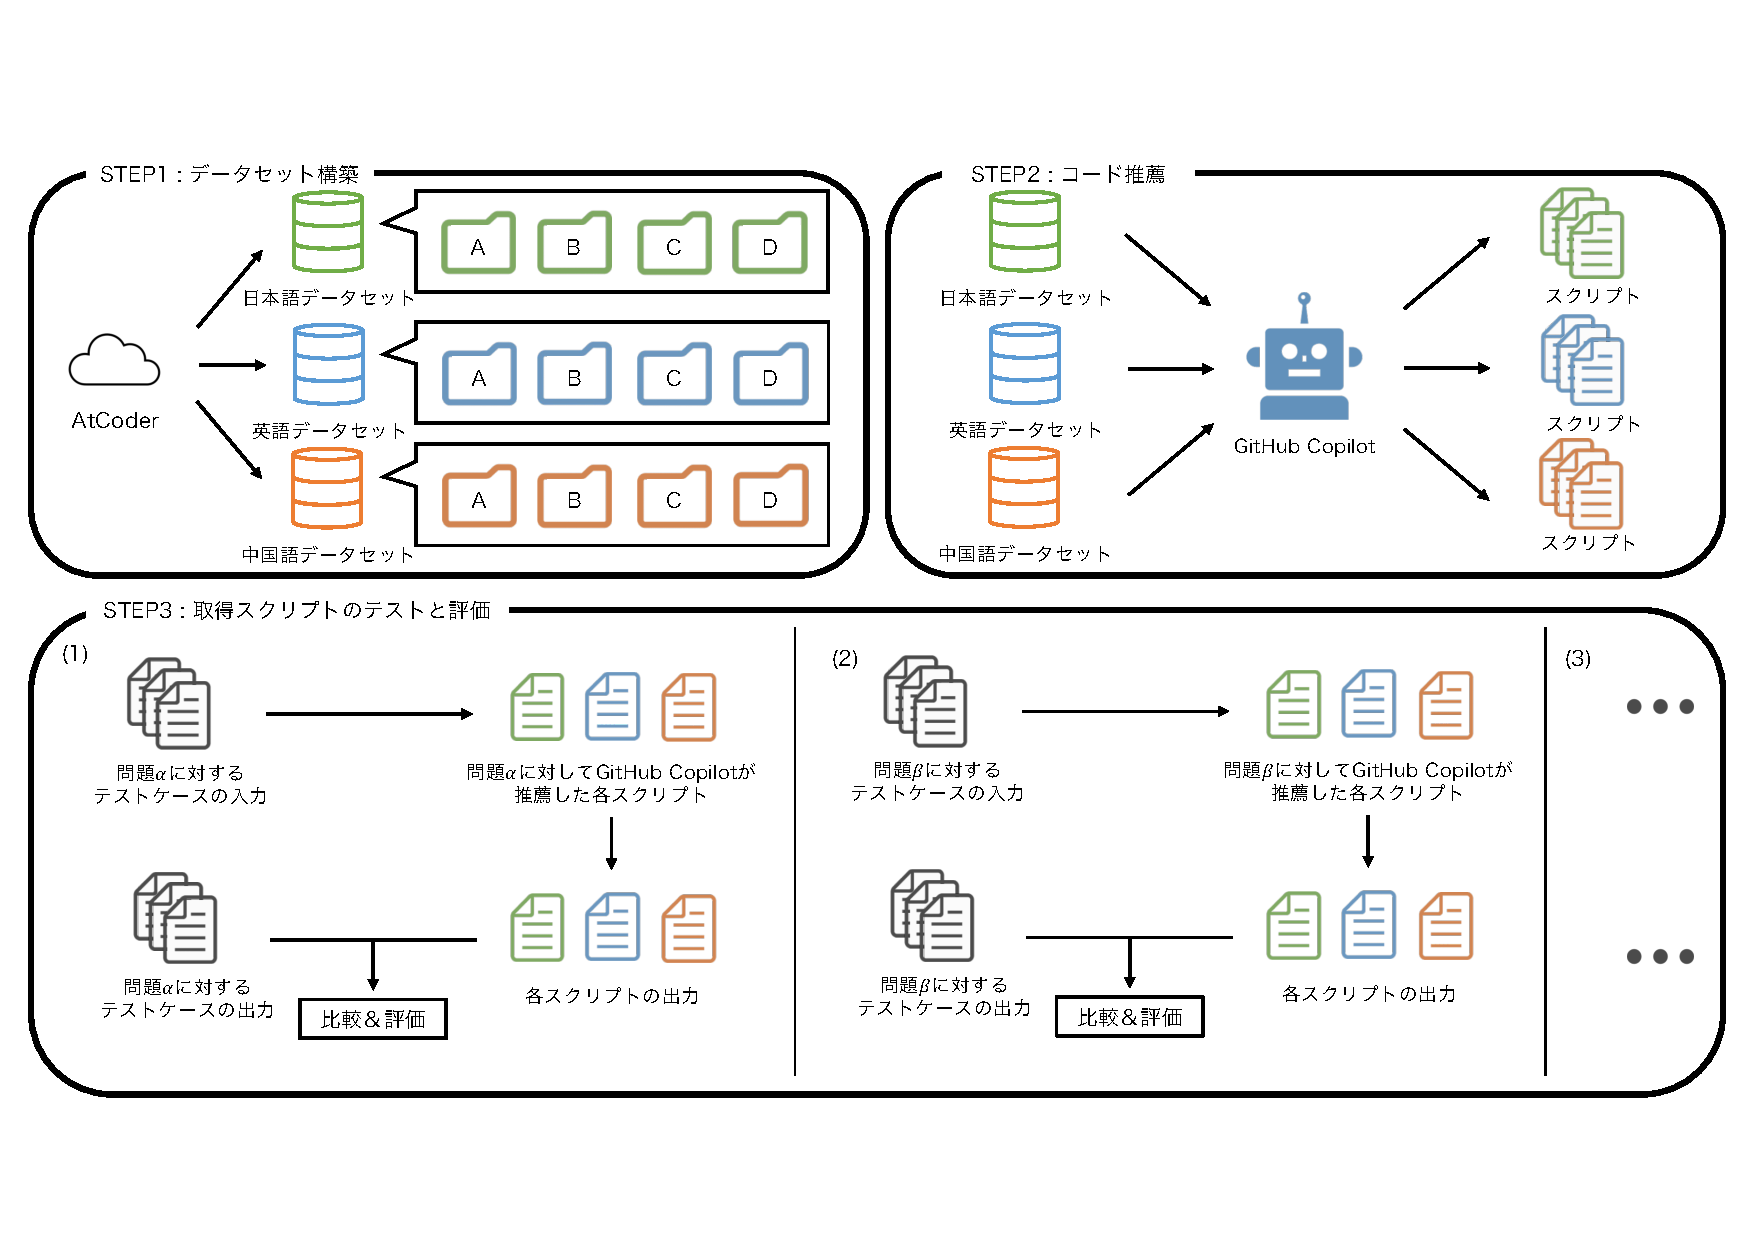
\includegraphics[width=\linewidth]{image/system.pdf}
    \caption{実験設計の概要}
    \label{experiment_design}
  \end{figure}
  
  \subsection{データセット構築\label{build_dataset}}
    本研究では日本国内において最大の競技プログラミングコンテストであるAtCoder\cite{AtCoder}の問題を使用する.
    中でも,AtCoder Beginner Contestという毎週開催されているコンテストの問題を使用する.
    このコンテストは6/24までに1${\sim}$307(2023/06/24現在)の問題が公開されており,
    各問題の難易度はA, B, C, D, E, F, G, Ex(H)までの最大8段階でアルファベットの語順が後になるほど難易度が高くなる.
    また,問題は日本語版と英語版が準備されている.
    この問題から,問題番号99${\sim}$287,各問題の難易度A${\sim}$Dの日本語版および英語版を使用する.
    問題を限定する理由としては,
    問題番号は十分なテストケースの数が確保されている問題を使用するため,
    問題難易度は事前実験にてCopilotが正しいプログラムを生成できる境目であったためである.
    続いて,中国語版の問題はAtCoderには存在しないため,
    英語版のデータセットをDeepL APIを使用して翻訳し,
    翻訳した問題をネイティブによる校正を行うことで,中国語版のデータセットを作成した.
    最終的に,問題番号が99${\sim}$287,各問題の難易度がA,B,C,D,問題の言語が英語,日本語,中国語の三つのデータセットが取得でき,
    これらを本実験のデータセットとした.

  \subsection{プログラム推薦\label{recommend_program}}
    \ref{build_dataset}節で作成したデータセットに対して,Copilotでプログラム推薦を行う.
    \ref{build_dataset}節で作成した各言語のデータセットの中には,問題番号が99${\sim}$287,各問題の難易度がA,B,C,D存在するため,合計で2,268問存在する.
    これらの問題に対して,プログラム推薦を行う.
    
    \begin{table}[t]
      \caption{問題212-Aの日本語版}
      \begin{tabular}{c}
        \begin{tabularx}{23zw}{X}
          \hline
          \verb|問題文| \\
          \verb|高橋くんは A グラムの純金と B グラムの純銀| \\
          \verb|(0 ≦ A,B, 0 < A+B) をよく溶かした上で混ぜ合わせ、新たな金属を生成しました。| \\
          \verb|生成された金属は「純金」「純銀」「合金」のいずれでしょうか?| \\
          \verb|なお、生成された金属は|
          \verb|0 < A かつ B=0 なら「純金」| \\
          \verb|A=0 かつ 0 < B なら「純銀」| \\
          \verb|0 < A かつ 0 < B なら「合金」| \\
          \verb|であるとみなします。| \\
          \verb|制約| \\
          \verb|0 ≦ A,B ≦ 100| \\
          \verb|0 < A+B| \\
          \verb|A,B は整数| \\
          \verb|入力| \\
          \verb|入力は以下の形式で標準入力から与えられる。| \\
          \verb|A B| \\
          \verb|出力| \\
          \verb|生成された金属が「純金」なら Gold と、| \\
          \verb|「純銀」なら Silver と、「合金」なら Alloy と出力せよ。| \\
          \verb|入力例 1| \\
          \verb|50 50| \\
          \verb|出力例 1| \\
          \verb|Alloy| \\
          \verb|入力例 2| \\
          \verb|100 0| \\
          \verb|出力例 2| \\
          \verb|Gold| \\
          \hline
        \end{tabularx}
      \end{tabular}
      \label{problem_212_A_en}
    \end{table}

    表\ref{problem_212_A_en}は問題102-Aの英語版のデータセットの中身である.
    このように各問題のデータセットには,問題,制約,入力,出力,サンプル入力,サンプル出力がコメントとして記述されている.
    ただし,問題によってサンプル入力およびサンプル出力の数は異なり,また注釈等の記述がある場合もある.
    このデータセットを入力として,Copilotによるプログラム推薦を行い,$x$個の推薦プログラムを得る.
    このとき,$x$は$0 {\leq} x {\leq} 10$を満たす.
    また,推薦プログラムで出力するプログラミング言語はPythonを使用した.
    この入力から出力までの流れを各問題に対して5回実行する.
    その理由としては,Copilotの推薦スクリプトが毎回変化するため,
    このランダム性を考慮して,評価を行うためである.
    
  \subsection{取得プログラムのテストと評価\label{test_and_evaluation}}
    \ref{recommend_program}節で取得したプログラムに対して,テストを行う.
    このテストは,各問題に対して,テストケースの入力を入力として取得したプログラムを実行し,テストケースの出力と一致するかを確認する.
    そして,各推薦スクリプトが全てのテストケースを通過したか否かで評価を行う.
    使用した評価指標は,$Accuracy$(正答率)で,推薦された全スクリプトの内,全てのテストケースを通過したスクリプトの割合を示す.


